\documentclass[a4paper]{scrreprt}

\usepackage{amsmath}
\usepackage{amssymb}
\usepackage[ngerman]{babel}
\usepackage[T1]{fontenc}
\usepackage[utf8]{inputenc}
\usepackage[svgnames]{xcolor}
\usepackage[scaled]{helvet}
\usepackage{graphicx}
\usepackage[final]{pdfpages}
\usepackage{caption}

%\title{Solutions to ICP Exercises}
%\author{Rico Häuselmann}

\begin{document}
%\maketitle

\chapter*{Exercise 1}

\section*{Model}
The Ising model is represented by a 3-dimensional lattice of $L^3$ integer values $\sigma_{ijk}$. 
For a given temperature $N_S\cdot L^3$ single spin flips at random positions are performed.
The temperature of the system is raised in steps of $\delta T = \left(T_e - T_s\right) / N_T$.
The program takes $L$, $T_s$, $T_e$, $N_T$, $N_S$ as parameters.

Energy and magnetization are measured as $\frac{E^{(T)}_{tot}}{J} = \sum_nn \sigma_{a} \sigma_{b}$ and
$M^{(T)}_{tot} = \sum_{ijk} \sigma_{ijk}$ respectively.
Those quantities are measured after each $L^3$ single spin flips (a ``system sweep'') and 
subsquently averaged over all $N_S$ sweeps of a timestep giving $\left<E_{tot}\right>_T$ and 
$\left<M_{tot}\right>_T$.

Utilizing the same scheme $\left<E^2_{tot}\right>_T$ and $\left<M^2_{tot}\right>_T$ are retrieved.
Using these quantities $\chi (T) = \frac{ \left<M^2_{tot}\right>_T - \left<M_{tot}\right>_T^2 }{T}$
as well as $C_V(T) = \frac{ \left<E^2_{tot}\right>_T - \left<E_{tot}\right>^2 }{T^2}$ can be computed.

All four quantities are then given out per system size $L^3$.

\section*{Code}
The code can easily be built using cmake. run \verb*|\$ cmake . && make| in the directory ex01\_ricoh/src/Ex1/. Or run the script run\_experiments.sh which builds the code, writes the parameter files and starts the program.

\section*{Simulations}
The following value was found to lead to converging simulations: $N_S = 200$.
Temperature was varied from $T_s = 0$ to $T_e = 8$ in $N_T = 100$ steps.
The experiment was run for systems of the size $L = \left\{10, 15, 20, 25\right\}$.

\section*{Results}

All quantities were plotted vs. $T$ for all system sizes. Additionaly the theoretical value for $T_c = 4.51$
was plotted as a vertical line.

\begin{figure}[h!]
    \begin{center}
        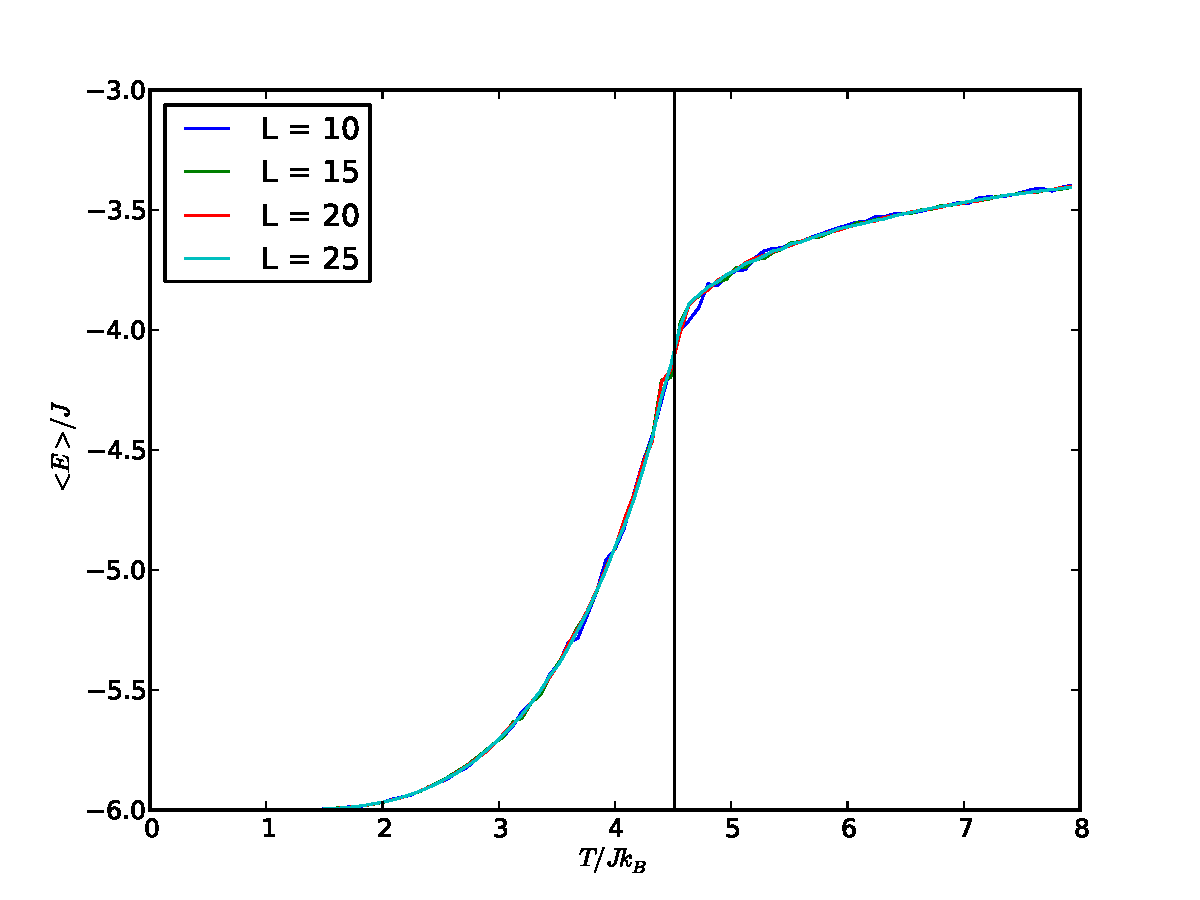
\includegraphics[width=0.9\textwidth]{energy} \\
        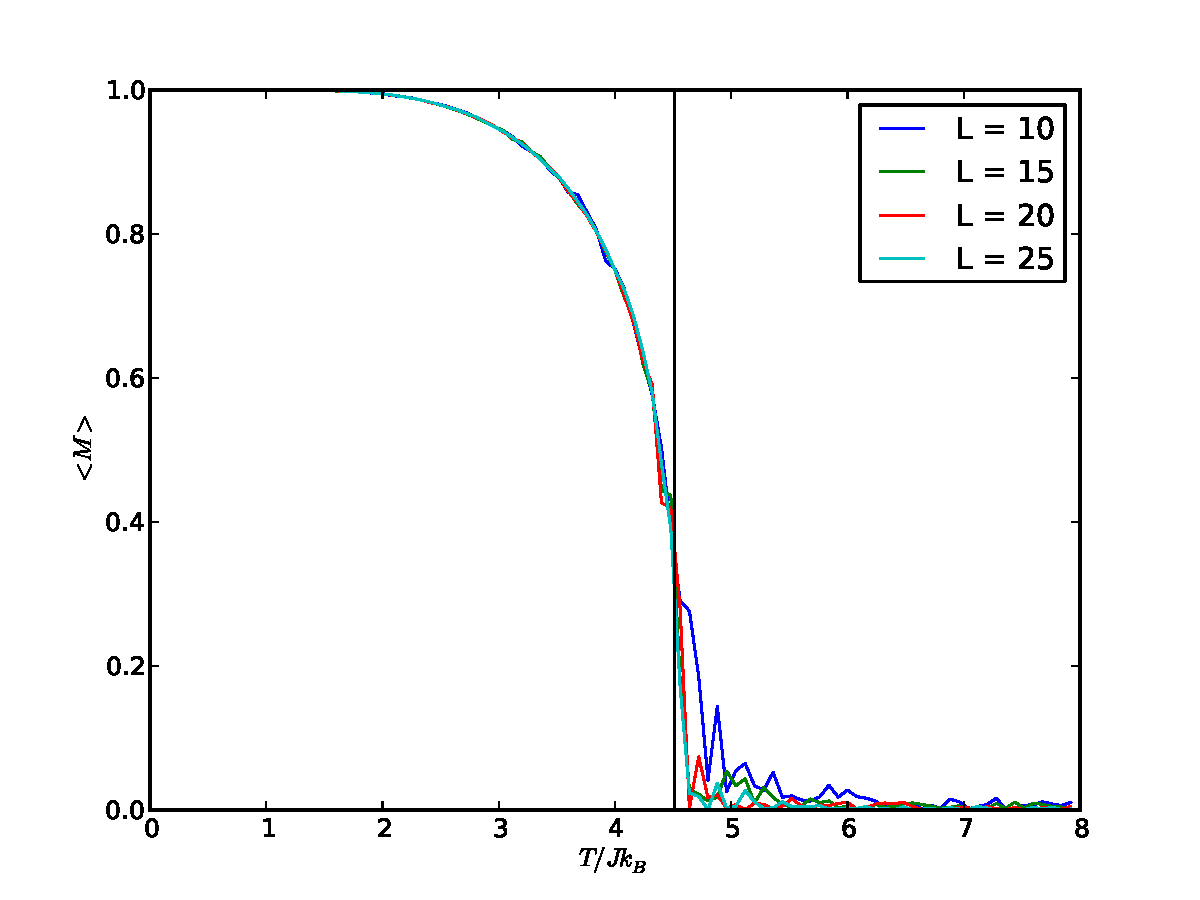
\includegraphics[width=0.9\textwidth]{magnetization}
    \end{center}
    \caption*{The Energy increase flattens after $T=T_c$. 
            Magnetization should decrease exponentially until reaching 0 at $T_c$.
            The higher $L$ gets the less $\left<M\right>$ will fluctuate after $T_c$.}
    \label{fig:ex6res}
\end{figure}

\begin{figure}[h!]
    \begin{center}
        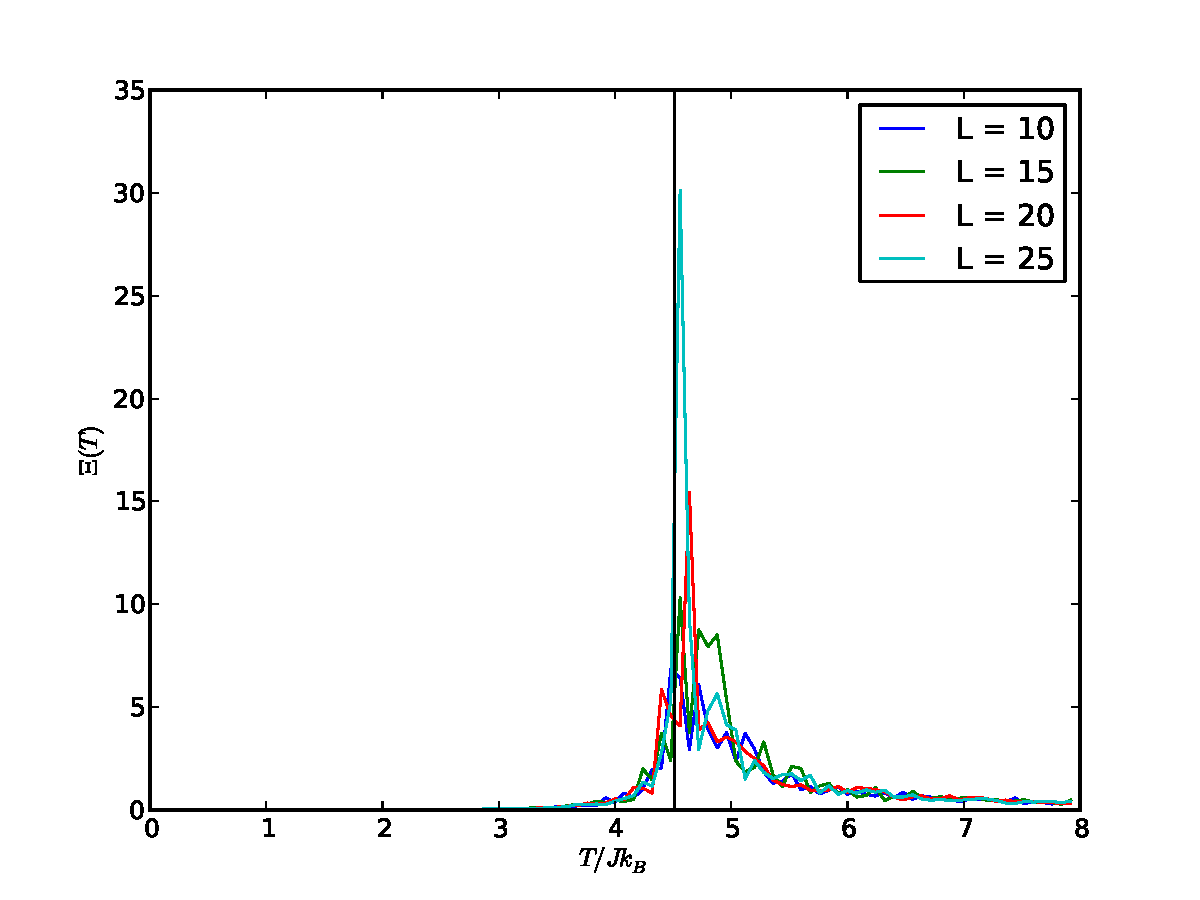
\includegraphics[width=0.9\textwidth]{xi} \\
        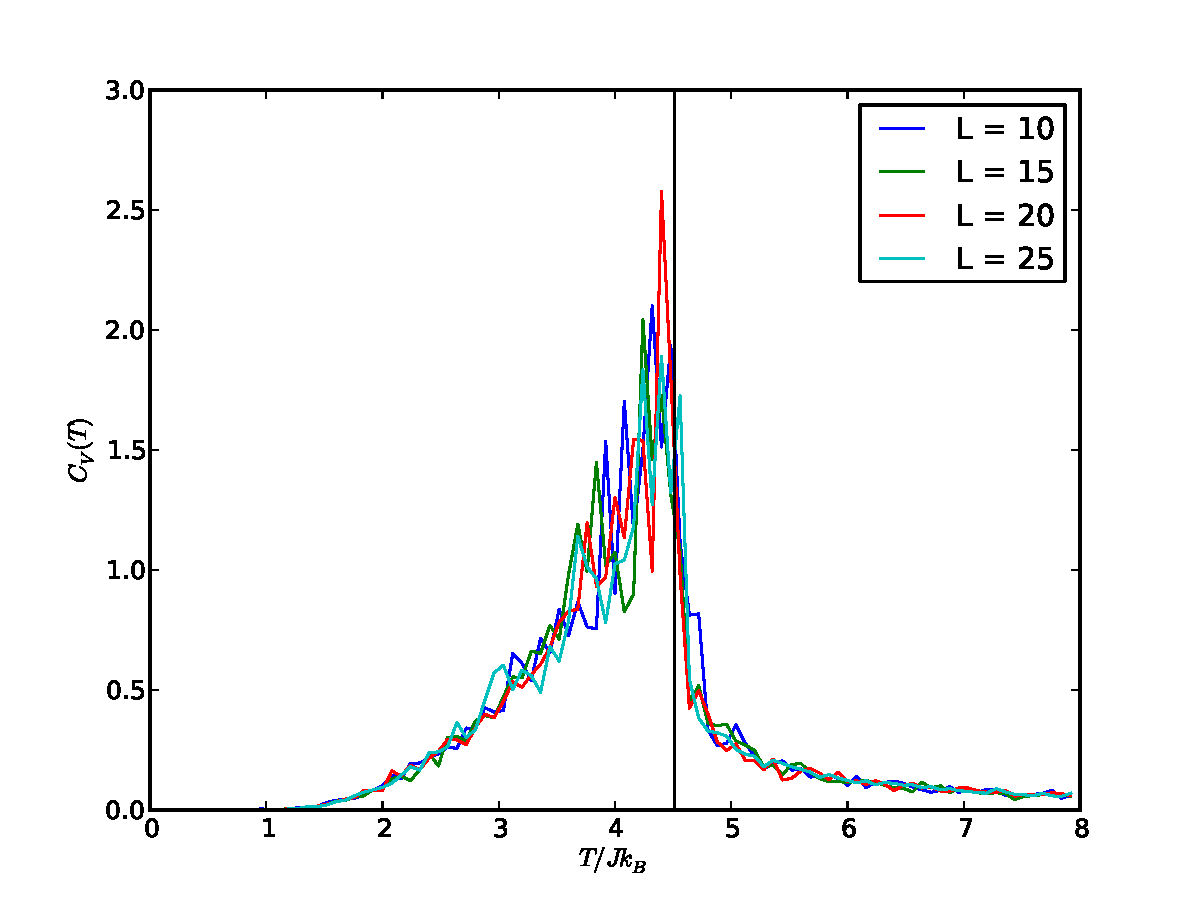
\includegraphics[width=0.9\textwidth]{cv}
    \end{center}
    \caption*{These two quantities should display a pole at $T_c$ which they do for high enough $L$.}
    \label{fig:ex6res}
\end{figure}

\end{document}

